\documentclass[a4paper, 12pt]{article}
\usepackage[francais]{babel}
\usepackage{graphicx}
\usepackage[utf8]{inputenc}
\usepackage[T1]{fontenc}
\usepackage{fancyhdr}
\usepackage[margin=1in]{geometry}
\usepackage{amsmath}
\usepackage{amssymb}
\author{Thibault \bsc{BEZIERS LA FOSSE}}
\date{}
\title{Étude et Comparaison d'Algorithmes}



\pagestyle{fancy}
\begin{document}

\maketitle
\clearpage

\tableofcontents
\clearpage

\section{Introduction}
Ce projet en six séances à pour objectif d'implémenter des algorithmes, afin de calculer leurs complexités et comparer les performances. 
Quatre algorithmes sont à notre disposition, ce compte rendu les traitera dans l'ordre donné. Seront expliqués:
\begin{itemize}
\item[L'implémentation]
\item[La complexité théorique]
\item[Les résultats d'exécutions]
\item[L'analyse des résultats]
\item[Le comparatif des résultats théoriques et expérimentaux]
\end{itemize}
\subsection{Objectif}
Les quatre algorithmes à implémenter consistent à trouver la suite de termes du tableau dont la somme est maximum. 
Les éléments du tableau sont choisis de manière aléatoire, et nous exécuterons nos algorithmes sur des tableaux de tailles variables, en commençant par des tableaux de moins d'une dizaine d'éléments, à des tableaux qui en contiennent des dizaines de milliers.  
\subsection{Outils utilisés}
Le langage de programmation à utiliser pour ce projet étant libre, j'ai choisi de m'orienter vers le C++. D'abord pour une raison pratique, l'université nous fait régulièrement utiliser ce langage. Ensuite pour des raisons de performances, car C++ reste un langage assez efficace pour effectuer des opérations comme celles de ce projet.
Le compilateur utilisé est G++, avec la librairie C++11. Effectivement, G++ est disponible à l'université, et la librairie C++11 offre des méthodes efficaces, et surtout pratiques pour manipuler des tableaux. 

Afin de rendre mon programme plus simple à utiliser, j'ai aussi implémenté une interface graphique avec Qt. Les deux sont utilisables, et les instructions d'installation sont détaillées dans le fichier README.md à l'intérieur de la racine du projet. 
\subsection{Structure du programme}
Quatre algorithmes étant à implémenter, j'ai choisi de créer une arborescence de classes sur un seul niveau. En haut, une classe abstraite implémentant les principales méthodes nécessaires à l’exécution des algorithmes, et en bas les algorithmes qui redéfinissent la méthode de calcul de la méthode \bsc{MaxSomme}:

\begin{figure}[h]
	\centering
	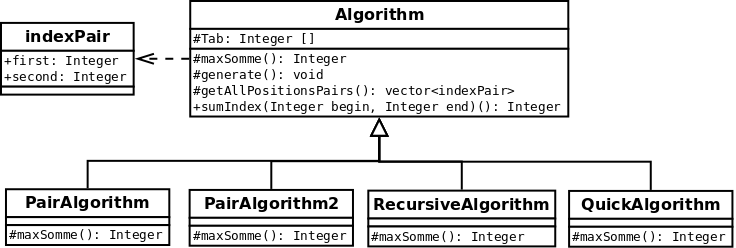
\includegraphics[scale=0.3]{diagramme.png}
	\caption{Diagramme UML du programme}
	\label{uml}	
\end{figure}

 
Les algorithmes implémentés doivent calculer la différence entre deux cases du tableau. J'ai décidé de créer une structure très simple, appelée IndexPair, contenant deux entiers: first et second, contenant chacun une cellule du tableau:
\begin{verbatim}
struct {
    int first;
    int second;
}
\end{verbatim}

\subsection{Méthodes principales}
Voici les méthodes, ainsi que leurs complexités respectives, qui sont implémentées dans la classe mère pour être ensuite réutilisées dans tous les algorithmes.
\subsubsection{Méthode: generate(Int n): void}
Cette méthode remplit le tableau avec des nombres aléatoires entre -1000 et 1000. Le paramètre $n$ correspond au nombre de cases désirées pour le tableau, et l'algorithme est très simple:
\begin{verbatim}
Pour i allant de 1 à n:
    tab[i] = random(-1000, 1000)
FinPour
\end{verbatim}
La complexité de la fonction random étant constante, cette méthode a une complexité en $\theta (n)$.

\subsubsection{Méthode: getAllPositionPairs()}
Cette méthode calcule toutes les paires possibles en fonction de la taille du tableau. Par exemple pour un tableau [1, 2, 3, 4], elle renverra un tableau qui contient les paires {[1,2], [1, 3], [1, 4], [2, 3], [2, 4], [3, 4]}
L'algorithme est le suivant:
\begin{verbatim}
Paires = []                         Coût: 1 
Pour i allant de 1 à n-1:           Coût: Voir ci-dessous
    Pour j allant de i+1 à n:       Coût: Voir ci-dessous
        Paires.ajouter([i, j])      coût: 1
    FinPour
FinPour
\end{verbatim}
Cet algorithme est assez simple à implémenter, et nécessaire pour plusieurs des algorithmes de MaxSomme. 
Détail du calcul de sa complexité théorique:

Boucle 1: effectuée $n-1$ fois

Boucle 2: effectuée $(n-2) + (n-3) + (n-4) + ... + n-(n-1)$ fois
soit $1 + 2 + ... + n-2$

Ainsi on a la somme des entiers de 1 à n-2 qui peut être calculée ainsi:

\begin {center}
$\frac{(n-3)(n-2)}{2}$
\end{center}

Sans détailler le calcul, on voit immédiatement qu'on a un produit de $n$, on peut donc en déduire une complexité en $\theta(n^2)$.

\subsubsection{Méthode: sumIndex(Int a, Int b): int}
Cette méthode est simple, elle prend deux entiers en paramètre, qui sont chacun un indice du tableau, et calcule la somme des cases du tableau entre ces deux indices. Cet algorithme est récursif:
\begin{verbatim}
Si debut == fin:
    Retourner fin
Sinon 
    Retourner tab[debut] + sumIndex(debut+1, fin)
Fin
\end{verbatim}
On a une complexité en $\omega(1)$ si on désire la somme entre les deux mêmes cellules, et en $O(n)$ pour une somme du début à la fin du tableau.
\section{Algorithme 1 : PairAlgorithm}
\subsection{Implémentation}
Cet algorithme est facile à implémenter et repose surtout sur les principales méthodes de la classe mère $Algorithm$:
\begin{verbatim}
paires = getAllPositionPairs()
max = NaN
pour chaque paire p:
    courant = sumIndex(p.first, p.second)
    si max == NaN ou courant < max:
        max = courant
    fin si
fin pour
retourner max
\end{verbatim}
L'implémentation en $C++$ est visible dans le programme ci-joint.
\subsection{Complexité théorique}
La complexité de cet algorithme repose sur la complexité des méthodes utilisées. 
On utilise la méthode \emph{getPositionPairs} qui est en $\theta(n^2)$ et pour chaque résultat obtenu on effectue une méthode en $O(n)$  : \emph{SumIndex}.
On peut donc en déduire que la complexité finale de cet algorithme est en $O(n^3)$

\subsection{Résultats d’exécutions}
L'algorithme a été exécuté sur des tableaux de taille variable, de 1 à 4000 éléments, en augmentant progressivement le pas. On obtient les résultats suivants:

\begin{minipage}[c]{0.4\linewidth}
   \begin{tabular}{|l|c|}
      \hline
      Taille & Temps (millisecondes) \\
      \hline
   100	& 0 \\
   200	& 1\\
   300	& 4\\
   500	& 11\\
   800	& 28\\
   1000	& 42\\
   1500	& 109\\
   2000	& 221\\
   2500	& 417\\
   3000	& 703\\
   3500	& 1084\\
   4000	& 1579\\
   5000	& 3023\\
   7000	& 8172\\
   8500	& 14289\\
   10000 & 	23105\\
   12000& 	39960\\
   13500& 	56736\\
   14000& 	PAR\\
   \hline
   \end{tabular}
\end{minipage}\hfill
\begin{minipage}[c]{0.6\linewidth}
	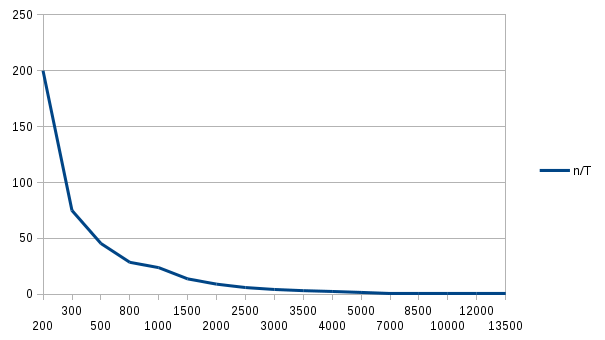
\includegraphics[scale=0.6]{curve_algo_1.png}
 	Voici la courbe obtenue en calculant le rapport $t/n$. Elle augmente très rapidement avec la taille des données, on peut en déduire une complexité polynomiale en la taille des données, au moins. Pour un tableau de 1000 données, on est à 42ms, et pour 2000, on est à 221ms. En multipliant les données par 2 ici, on multiplie le temps par 5. De 3500 à 7000, par 8. L'augmentation n'est clairement pas linéaire, elle est proche de $f(x) = x^3$.
\end{minipage}
\subsection{Analyse}
En observant les résultats d’exécution, on peut clairement voir que le temps augmente très rapidement à partir de $n=100$. On ignore les valeur antérieure car la vitesse d’exécution de l'algorithme est instantanée sur des données inférieures. En observant la courbe on remarque que la complexité temporelle correspond à la croissance de la fonction $f(x) = x^3$. Ainsi on peut affirmer que la complexité théorique calculée correspond à celle obtenue avec l'analyse de l'algorithme: $\theta (n^3)$.
\section{Algorithme 2: PairAlgorithm2}
\subsection{Implémentation}
Comme l'indique le sujet, cet algorithme fonctionne en deux temps. Dans un premier temps on remplit un tableau \bsc{SOMME} parallèle au tableau \bsc{Tab} qui, pour chaque cellule de \bsc{Tab} contient la somme depuis la première cellule, jusqu'à la cellule courante. Par exemple:

\begin{tabular}{|ccccccccc|}
\hline
\multicolumn{9}{|c|}{\bsc{Tab}} \\
\hline
Cellule: & 1& 2& 3& 4& 5& 6& 7& 8 \\
Valeur: & 3 & 4 & 8 & 9 & 2 & 1 & 4 & 5 \\
\hline
\end{tabular}

\begin{tabular}{|ccccccccc|}
\hline
\multicolumn{9}{|c|}{\bsc{Somme}} \\
\hline
Cellule: & 1& 2& 3& 4& 5& 6& 7& 8 \\
Valeur: & 3 & 7 & 15 & 24 & 26 & 27 & 31 & 36 \\
\hline
\end{tabular}

    \noindent De cette manière on peut aisément connaître la Somme entre deux indices du tableau en soustrayant la seconde somme à la première. Par exemple, pour connaître la somme des nombres entre la cellule 3 et la cellule 6 de \bsc{Tab} on peut soit faire:

    \noindent $8 + 9 + 2 = 19$ avec le tableau \bsc{Tab} comme avec l'algorithme \emph{PairAlgorithm}. 

    Ou alors :

    \noindent $26 - 7 = 19$ avec le tableau \bsc{Somme}.

    \noindent On a donc comme méthodes:
\subsubsection{CalculateSommeTab}
\begin{verbatim}
Somme = []
current = 0
pour i allant de 1 à taille de Tab:
    current += Tab[i]
    Somme[i] = current
finPour
retourner Somme
\end{verbatim}
L'algorithme consiste à faire un parcours du tableau, et à sommer les cellules précédentes à la courante. La complexité est en $\theta(n)$, puisque l'on ne fait qu'un unique parcours du tableau.
\subsubsection{MaxSomme}
\begin{verbatim}
Somme = CalculateSommeTab()
Paires = getAllPositionPairs()
Max = NaN
Pour chaque paire p de Paires:
    si p.first = 1
        courant = Somme[p.second]
    sinon
        courant = Somme[p.second] - Somme[p.first]
    finSi
    si courant > max || max = NaN
        max = courant
    finSi
FinPour	
\end{verbatim}
\subsection{Complexité Théorique}
\emph{CalculateSommeTab} a une complexité en $\theta(n)$. On retrouve ici la méthode \emph{getAllPositionPairs} dont on avait fixé la complexité à $\theta(n^2)$. Et pour chaque paires obtenues on effectue une opération en $\theta(1)$. On peut donc déterminer une complexité en $\theta(n^2)$ pour cet algorithme. On gagne un ordre de grandeur par rapport à l'algorithme précédent, qui devrait se ressentir lors des résultats d’exécution. 
\subsection{Résultats d’exécution}
On exécute le programme sur des tableaux de taille de plus en plus grande. On s'arrête lorsque le programme est trop lent, ou la mémoire de l'ordinateur ne suffit pas. On obtient ainsi les résultats suivants:

\begin{minipage}[c]{0.4\linewidth}
\begin{tabular}{|c|c|}
\hline
Taille & Temps(millisecondes) \\
\hline
100	& 0\\
200	& 1\\
300	& 2\\
500 & 6\\
800& 	10\\
1000& 	12\\
1500& 	18\\
2000& 	32\\
3000& 	51\\
4000& 	80\\
5000& 	124\\
7000& 	245\\
10000& 	479\\
15000& 	1038\\
20000& 	1870\\
30000& 	4098\\
40000& 	7450\\
45000& 	8989\\
50000& 	DM\\
\hline
\end{tabular}
\end{minipage}\hfill
\begin{minipage}[c]{0.6\linewidth}
	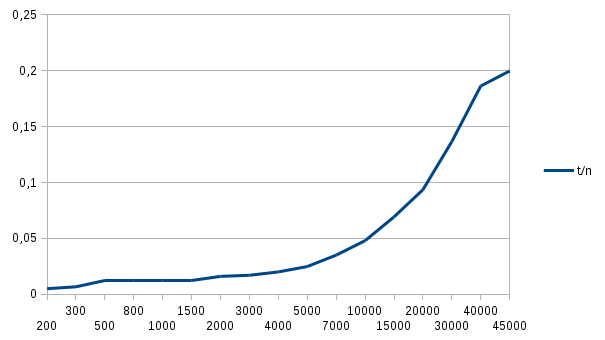
\includegraphics[scale=0.6]{curve_algo_2.png}
	 	Voici la courbe obtenue en calculant le rapport $t/n$. On remarque rapidement que l'augmentation est moins forte que celle du premier algorithme. On peut donc déjà penser que la complexité sera au plus équivalente. De 5000 à 10 000, on multiplie par un facteur 3.8. De 15 000 à 30 000, par un facteur 3.9, et de 20 000 à 40 000 par 3.95. Quand on double la taille des données, on multiplie par 4 le temps. On peut tout de suite penser à une complexité $f(n) = n^2$.
\end{minipage}\hfill
\subsection{Analyse}
La première chose que l'on puisse dire, c'est ce que cet algorithme est nettement plus efficace que le précédent. Effectivement, on s'arrête parce que la mémoire de l'ordinateur ne suffit plus. Sans ça le temps d’exécution pour un tableau de taille $n=45000$ reste tout à fait correct par rapport a ce qu'on a eu précédemment. On voit bien que le temps d’exécution augmente de plus en plus vite en fonction de la taille des données, on a bien une correspondance avec la complexité théorique calculée: $\theta(n^2)$.


\section{Algorithme 3: Recursive Algorithm}
\subsection{Implémentation}
Des quatre algorithmes à implémenter, celui-ci a la complexité la plus compliquée à calculer, de par la longueur de l'algorithme, mais aussi à cause de sa récursivité. L'algorithme intéressant est dans la méthode \emph{calcul3}, que l'on appelle dans la méthode \emph{maxSomme} sur un tableau de taille $n$:
\subsubsection{MaxSomme}
\begin{verbatim}
retourner calcul3(1, n)
\end{verbatim}
\subsubsection{calcul3}
La méthode \emph{calcul3} fonctionne en quatre temps. Tout d'abord on a deux conditions d'arrêt: Lorsque la cellule de début est après la cellule de fin, ou lorsque la cellule de début et celle de fin est la même.
\begin{verbatim}
si (début > fin):
    retourner 0
fin si

si (début == fin):
    si (tab[début] > 0):
        retourner tab[début]
    sinon
        retourner 0
    fin si        
fin si   
\end{verbatim}
Si la cellule de début est après la cellule de fin, c'est qu'on a une incohérence lors de l'appel de la méthode, et que son utilisation n'est pas respectée. Ainsi on s'arrête en retournant 0. Enfin si la cellule de début et celle de fin est la même, c'est que la somme maximum entre les deux n'a pas à être calculée, et dans ce cas on retourne 0 si l'indice est inférieur à 0 (ce n'est pas un maximum, c'est négatif), ou bien on retourne l'indice en question.
La suite de l'algorithme consiste à prendre la cellule située au milieu du tableau, puis à calculer la somme entre la cellule du début et celle du milieu, et entre celle du milieu et celle de la fin et enfin de calculer le maximum entre-elles.
Ainsi on a :
\begin{verbatim}
milieu = (debut+fin)/2
maxGauche = 0
somme = 0
i = milieu
tant que i >= début:
    somme += tab[i]
    maxGauche = Maximum(somme, maxGauche)
    i--
fin tant que 
\end{verbatim}
On somme tous les éléments du début au milieu, et on garde le maximum.
\begin{verbatim}
maxDroit = 0
somme = 0
i = milieu + 1
tant que i <= fin:
    somme += tab[i]
    maxDroit = Maximum(somme, maxDroit)
    i++
fin tant que 
\end{verbatim}
Même chose, sauf qu'on somme tous les éléments du milieu à la fin, et on garde le maximum.
Enfin on calcule le maximum entre \emph{maxDroit + maxGauche}, et la fonction appelée à nouveau sur la partie gauche et la partie droite du tableau.
\subsection{Complexité Théorique}
Ici la complexité dépend du nombre d'exécution de l'algorithme. On calcule succinctement la complexité pour un tableau de taille n = 8:
\begin{verbatim}
n
+ 2*(1/2)*n   --> Méthode appelée une fois sur chaque demi tableau (de taille 1/2*n = 4) --> 2 appels
+ 4*(1/4)*n   --> Méthode appelée une fois sur chaque quart de tableau (de taille 1/4*n = 2) --> 4 appels
+ 8+(1/8)*n   --> Méthode appelée une fois sur chaque huitième de tableau (de taille 1/8*n = 1) --> 8 appels
\end{verbatim} 
Enfin, comme le tableau est de taille 1, on s'arrête là. 
On a donc un coût de $4n$, comme $n = 8$, on a $1/2n*n = 32$. On peut alors s'attendre à une complexité supérieure à $n$ mais inférieure à $n^2$. 
Plus spécifiquement, \emph{calcul3} est en $\Omega(n)$ et en $O(n^2)$.

Dans cas général, pour un tableau de taille $n$ on appellera la fonction sur des demi-tableaux jusqu'à ce que $n$ soit réduit à 1. C'est à dire qu'on va faire des divisions successives de $n$ par $2$, jusqu'à 1: 
$log _2  n$ divisions. 

Chaque sous tableau est parcouru une fois, plus une fois pour le tableau de taille n, on calcule ainsi une complexité de:

$n + (log _2 n)*n $
$(1 + log _2)*n $

On en déduit une complexité théorique en notation de Landau de $\theta(nlog(n))$.
\subsection{Résultats d’exécution}
L'exécution sur un tableau de taille croissante donne les résultats suivants. On s'arrête lorsque le temps d'exécution de l'algorithme est trop long, ou bien lorsque l'on dépasse la mémoire de l'ordinateur.

\begin{minipage}[c]{0.4\linewidth}
\begin{tabular}{|c|c|}
\hline
Taille & Temps(millisecondes) \\
\hline
5000&	0\\
10000&	1\\
50000&	6\\
100000&	13\\
200000&	24\\
300000&	35\\
400000&	43\\
500000&	55\\
1000000&	104\\
2000000	& 211\\
3000000&	322\\
4000000	& 427\\
5000000	& 543\\
10000000&	1112\\
20000000&	2269\\
30000000&	3437\\
40000000&	4638\\
50000000&	5817\\
100000000&	11908\\
150000000&	18153\\
200000000&	24323\\
250000000&	30484\\
300000000 &  DM \\
\hline
\end{tabular}
\end{minipage}\hfill
\begin{minipage}[c]{0.5\linewidth}
	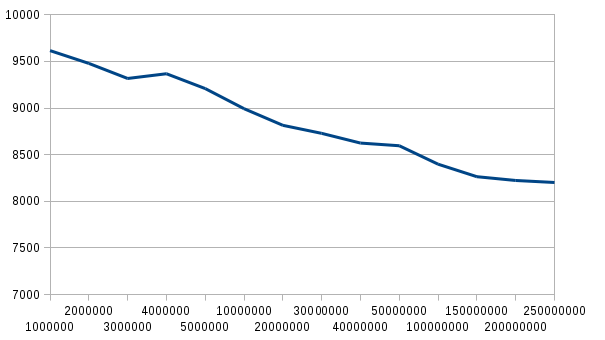
\includegraphics[scale=0.6]{curve_algo_3.png}
	
	
    Voici la courbe obtenue en calculant $t/n$
    La première partie est assez instable, néanmoins à partir de $n=10 000 000$, on a une légère croissance. Notre courbe étant celle de $t/n$, on peut en déduire que c'est un facteur qui augmente très légèrement, proportionnellement à $n$.
    On en déduit une augmentation de type $f(n) = n log n$.
\end{minipage}\hfill
\subsection{Analyse}
On a des résultats nettement meilleurs que l'algorithme 2, tant en temps qu'en mémoire.

Avec l'algorithme 2, pour un tableau de taille 45 000 on avait un temps d'exécution d'environ 9 secondes, alors qu'avec l'algorithme 3, pour un tableau de taille 50 000, on est à 55ms, c'est plus de 150fois mieux.
La complexité théorique calculée semble de plus correspondre avec les résultats d'exécution. On se rend bien compte ici, qu'avec une différence d'un ordre de grandeur, l'amélioration des performance est fulgurante. 
 
\section{Algorithme 4: Quick Algorithm}
\subsection{Implémentation}
Cet algorithme est tout petit en taille, et très efficace. C'est pour ça qu'il porte le nom de \emph{Quick Algorithm}. Son implémentation tient en quelques lignes, n'utilise aucune méthodes complexe:
\begin{verbatim}
a=0
b=0
i=1
Tant que i <= n faire:
    b = max(b+T[i], 0)
    a = max(a, b)
    i++
Fin TantQue
Retourner a
\end{verbatim}
Il est beaucoup plus simple à comprendre que le précédent: On fait un unique parcours du tableau, et tant que la somme des cellules successives est croissante on la conserve dans la variable b, et si cette valeur dépasse le maximum, on écrase le maximum avec cette nouvelle valeur.
\subsection{Complexité Théorique}
Cet algorithme n'effectue qu'un seul parcours du tableau, et pour chaque itération, n'effectue que des opérations en temps constant: deux additions, et deux maximums. 
La complexité obtenue est donc de $\theta(n)$. Le coût en espace aussi est maximum, puisque l'on ne stocke que le tableau lui même, et 3 variables entières (32 bits chacune), le coût en mémoire est donc aussi excellent.  
\subsection{Résultats d’exécution}
Voici les résultats d'exécution de l'algorithme 4. On commence avec des données de taille $n=10000$, puisque avec des données de taille inférieure, les temps d'exécution restent figés à 0. 

\begin{minipage}[c]{0.4\linewidth}
\begin{tabular}{|r|c|}
\hline
n & t(ms) \\
\hline
10000 &	0\\
20000 &	1\\
40000& 	2\\
50000 &	3\\
100000 &	5\\
500000	 & 20\\
1000000& 	39 \\
2000000&	77\\
3000000&	113\\
4000000&	147\\
5000000&	185\\
10000000&	367\\
50000000&	1788\\
100000000&	3556\\
150000000&	5491\\
200000000&	7132\\
250000000&	8832\\
300000000& DM\\
\hline
\end{tabular}
\end{minipage}\hfill
\begin{minipage}[c]{0.6\linewidth}
	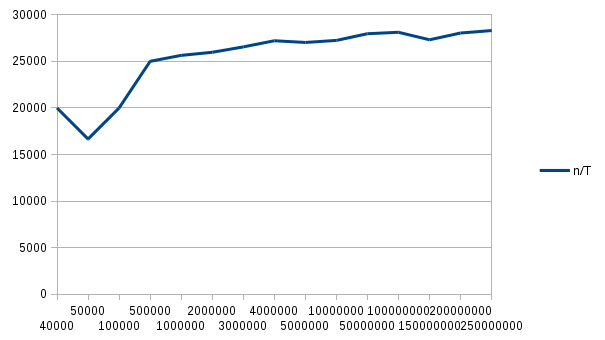
\includegraphics[scale=0.6]{curve_algo_4.png}
	 	Voici la courbe obtenue en calculant le rapport $t/n$. 
		On remarque que au début, les valeurs sont assez variables. C'est dû au peu de précision des données avec le chronomètre utilisé, il aurait fallu une précision au nanomètre ici pour avoir des valeurs justes.
		Néanmoins à partir de $n=500 000$ on remarque que la courbe est presque constante. On pourrait même croire qu'elle diminue. C'est à dire que le temps d'exécution augmente en même temps, et de manière linéaire à la taille des données. On a peut donc déterminer une complexité $f(n) = n$ avec cette courbe. 
\end{minipage}
\subsection{Analyse}
La courbe presque constante au dessus appuie la complexité théorique que nous avons calculé. On peut donc affirmer que la complexité de cet algorithme est en $\theta(n)$. 

\section{Conclusion}
Pour conclure ce projet, en implémentant et testant ces quatre algorithmes, on a pu voir l'importance de la complexité pour résoudre des problèmes. Effectivement, avec un algorithme efficace, on a pu traiter 250 000 000 de données, là où l'algorithme mauvais en traitait 7000. 

Ainsi avant de programmer le premier algorithme qui peut nous passer par la tête, il vaut mieux réfléchir à des méthodes plus efficaces, pour ainsi réduire de manière drastique nos temps de calculs. 
Enfin ce fût enrichissant de pouvoir mettre en pratique des connaissances vues en cours, et ainsi comprendre sur le fait accompli la différence de temps d'exécutions que peuvent avoir deux algorithmes résolvant le même problème.
\end{document}